\documentclass[10pt]{article}
\usepackage[letterpaper,landscape,margin=0.65in]{geometry}
\usepackage{graphicx}
\usepackage{booktabs}
\usepackage{amsmath}
\usepackage[T1]{fontenc}
\usepackage{hyperref}
\hypersetup{pdftitle={FROB C5 full quotient Frobenius map certificate},
  pdfsubject={EXP-FROB-91ee9c; full q-power matrix theorem; historical Sage review open}}
\setlength{\parindent}{0pt}
\setlength{\parskip}{0.45em}
\title{FROB C5 full quotient Frobenius maps}
\author{Validation audit, 22 October 2026}
\date{}
\begin{document}
\maketitle
\vspace{-2em}

\textbf{Scope.} For each frozen polynomial quotient over $\mathbf F_{11}$,
$\mathbf F_{13}$, or $\mathbf F_{19}$, Lean identifies the matrix of the
full $q$-power endomorphism in its power basis. This closes the gap
between previously proved basis-image coordinates and a linear-map matrix.

\begin{center}
\begin{tabular}{lll}
\toprule
Base field & Frozen quotient modulus & Matrix equality \\
\midrule
$\mathbf F_{11}$ & $z^5+2z^4+1$ & all $5\times5$ entries \\
$\mathbf F_{13}$ & $z^5+8z^4+1$ & all $5\times5$ entries \\
$\mathbf F_{19}$ & $z^5+3z^4+1$ & all $5\times5$ entries \\
\bottomrule
\end{tabular}
\end{center}

\textbf{Proof.} Mathlib's \texttt{frobeniusAlgHom} raises each quotient
ring element to its base-field cardinality and supplies an algebra
homomorphism, hence a base-field-linear map. Lean proves the quotient
moduli have degree five, uses the \texttt{AdjoinRoot} power basis, and
rewrites each \texttt{toMatrix} entry as the coordinate of the $q$-power
image of a basis monomial. The earlier exact quotient certificate proves
that coordinate equals the frozen matrix entry. All 75 full-map entries are
conjoined in one target theorem. No irreducibility assumption is needed for
this ring-level matrix calculation.

\textbf{Machine verification.} Source commit \texttt{1993b13e4a24} uses
pinned Lean 4.35.0-rc1. The exact-source verifier passed an 8,975-job full
build and 3,093-job target build. Its global audit found 667 theorem
declarations with standard axioms only; the requested theorem audit passed.
Independent semantic review remains pending.

\textbf{Boundary.} This is a mathematical quotient-algebra map result.
An additional Lean certificate proves the corresponding C5 controls for the
actual quotient q-power endomorphisms. Historical Sage field and kernel paths are not
proved to refine it; original
execution-source custody and independent code review remain open. The three
moduli have not been proved irreducible in Lean, although the independent
source-bound replay checks them. C8, the complete experiment gate, and
performance claims remain open. No trial or timing run was repeated.

\newpage
\begin{center}
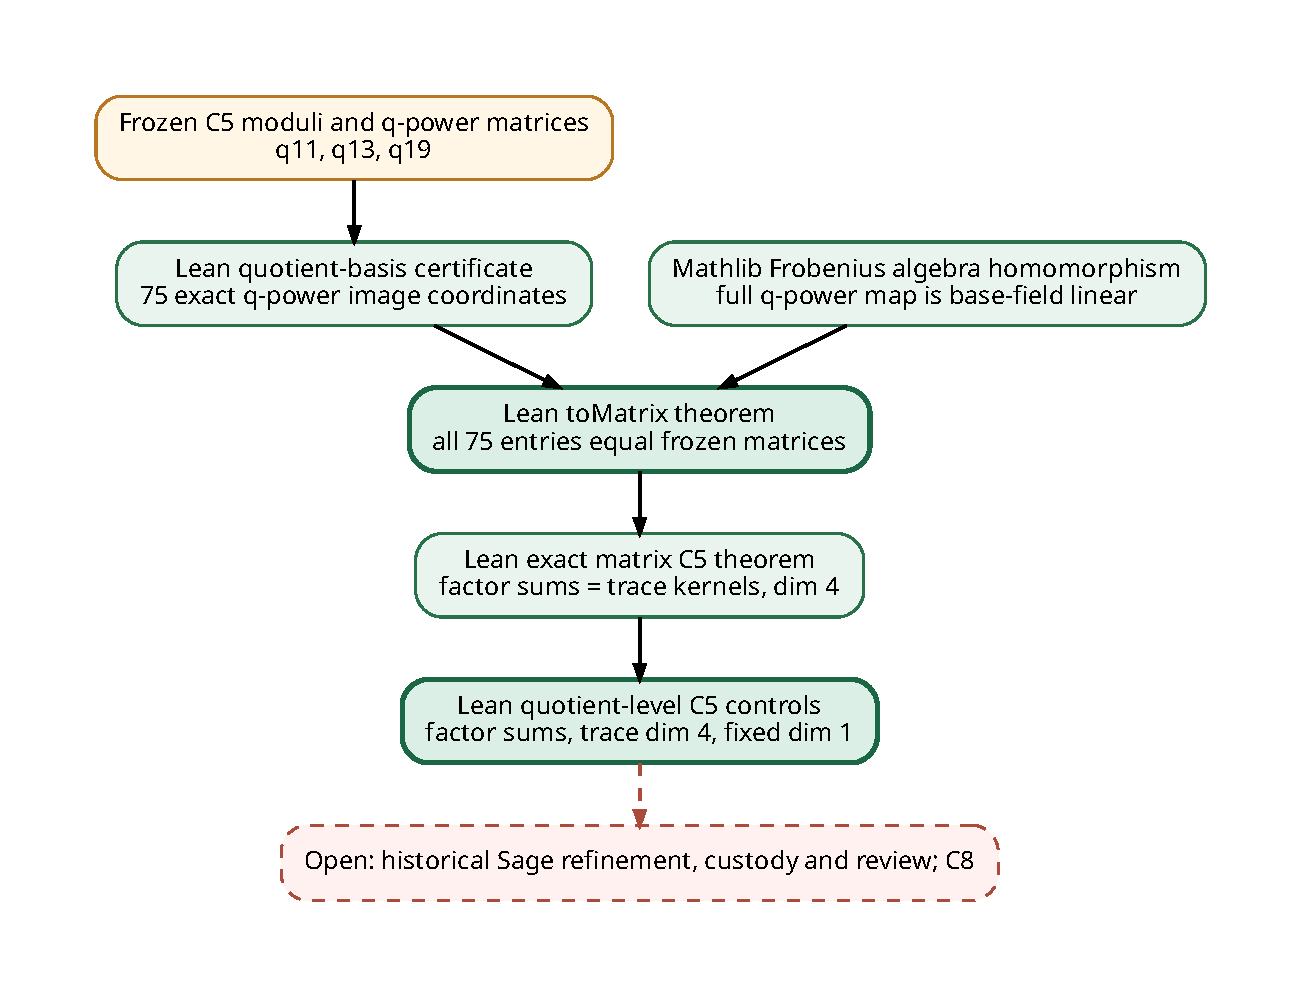
\includegraphics[width=\textwidth,height=0.82\textheight,keepaspectratio]{proof-figure.pdf}
\end{center}
\end{document}
